\documentclass[11pt]{article}
\usepackage{mathptmx}
\usepackage{setspace}
\usepackage{amsmath,amssymb}
\usepackage{amsthm}
\usepackage{fancybox}
\usepackage{algorithm, algpseudocode}
\usepackage{url}



\usepackage{enumitem}
\usepackage{multirow}
\usepackage{color}
\usepackage{graphicx}
\usepackage{setspace}
\usepackage{comment}
\usepackage{bm}


\begingroup
\renewcommand{\section}[2]{}%
%\renewcommand{\chapter}[2]{}% for othe

\newcommand*{\KeepStyleUnderBrace}[1]{%f
  \mathop{%
    \mathchoice
    {\underbrace{\displaystyle#1}}%
    {\underbrace{\textstyle#1}}%
    {\underbrace{\scriptstyle#1}}%
    {\underbrace{\scriptscriptstyle#1}}%
  }\limits
}

\usepackage{wrapfig}
\usepackage[margin=1in]{geometry}
 
\allowdisplaybreaks[4]
\usepackage{bbm}


\usepackage{amsrefs}
\usepackage{mathtools}
\mathtoolsset{showonlyrefs=true}


\usepackage[utf8]{inputenc}
\usepackage{hyperref}
\hypersetup{
    colorlinks=true,
    citecolor = blue,
    linkcolor=blue,
    filecolor=magenta,           
    urlcolor=cyan,
}

\usepackage[breakable, theorems, skins]{tcolorbox}
\DeclareRobustCommand{\mybox}[2][gray!20]{%
\begin{tcolorbox}[   %% Adjust the following parameters at will.
        breakable,
        left=0pt,
        right=0pt,
        top=0pt,
        bottom=0pt,
        colback=#1,
        colframe=#1,
        width=\dimexpr\textwidth\relax, 
        enlarge left by=0mm,
        boxsep=5pt,
        arc=0pt,outer arc=0pt,
        ]
        #2
\end{tcolorbox}
}

\theoremstyle{plain}
\newtheorem{thm}{Theorem}

\theoremstyle{definition}
\newtheorem{open}[]{Open problems}

 \usepackage[parfill]{parskip}
 
\usepackage[font=scriptsize,labelfont=bf]{caption}

\input macros.tex

\begin{document}
\begin{center}
\vspace{.2cm}
{\bf \large Beyond Matrices: Higher-order Tensors Methods in Machine Learning}\\
\end{center}
\vspace{.2cm}
\begin{itemize}[wide,noitemsep,topsep=0pt]
\item Principal Investigator Name and Job Title: Miaoyan Wang, Assistant Professor, UW-Madison
\item PI Phone Number and Email Address: 312-479-5123. miaoyan.wang@wisc.edu
\item Year Doctorate Awarded: 2015, University of Chicago
\item Number of Times Previously Applied: 0
\item Topic Area: Advanced Scientific Computing Research, Scalable Scientific Data Analysis and Reduction
\item Eligibility Extension Requested: No
\item FOA Number: DE-FOA-0002563
\end{itemize}


{\bf PI's qualification and prior supports.} I am currently a young female faculty member at UW-Madison and Institute for Foundations of Data Science, an NSF-funded multi-university initiative. I have a unique combination of post-graduate training in statistics (2010-2015, UChicago), mathematics (2015-2018, UPenn), and computer science (2015-2018, UC Berkeley). I use mathematical language in my work, and math steers my creation to understand the fundamentals of the problems. On the other hand, I feel mostly fulfilled when the developed tools help scientists to make discoveries in the domain field. During my career, I am fortunately to have worked closely with many fellow scientists on cutting-edge big data problems, which have shaped the scientific goals in this proposal. My previous work is supported by NSF on a different aspect of my research. I have not been supported by DOE grant before. 

{\bf Overview.} My proposed research is in the intersection of applied mathematics, machine learning, and optimization. Rapid developments in modern technologies have made multiway data readily available in daily lives. Tensor provides a generalized data structure in many learning procedures. %Methods built on tensors provide powerful tools to capture complex structures that lower-order methods fail to exploit. 
The empirical successes, however, are uncovering pressing new challenges that stand in the way of further progress: decisions arising from classical statistical premises are sensitive to model misspecification; greedy algorithms are yielding biased solutions; and concerns on prediction-interpretability balance continue to mount. {\bf The proposed project is to develop a suite of learning theory, scalable algorithms, and data-driven solutions for high-dimensional tensor problems.}

\begin{figure}[H]
\begin{center}
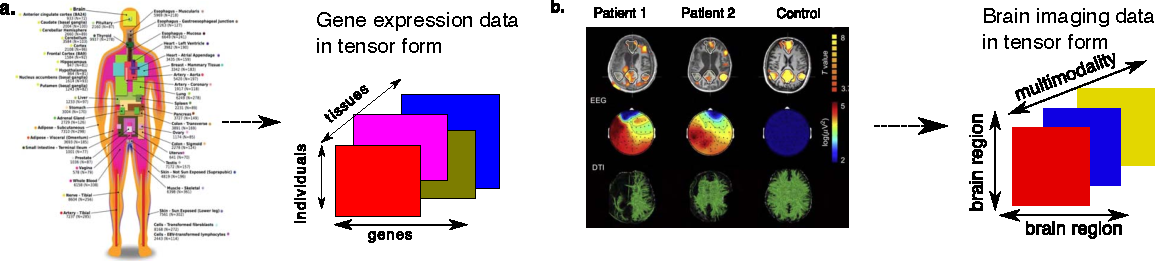
\includegraphics[width=1\textwidth]{example.pdf}
\caption{ \small (a) Examples of tensor data in scientific research. (a) GTEx data tensor consists of over 20,000 genes from 544 individuals across 53 human tissues. (b) HCP data tensor consists of multimodality connectivity measurements from over 1,200 individuals.}\label{fig:0}
\end{center}
\end{figure} 
\vspace{-.6cm}

{\bf Research questions.} Tensors are high-dimensional arrays. Recent advances in high-throughput sequencing technology have transformed scientific research into a data-intensive field where data are naturally generated in tensor form. One example of tensor data arising from my current collaboration is multi-tissue, multi-individual gene expression (Figure~\ref{fig:0}a). The completion of Genotype-Tissue Expression (GTEx) provides a huge compendium of tensor data consisting of millions of expression measurements from 20,000 genes across 544 individuals and 53 human tissues. Understanding the multifactorial patterns of whole-genome transcriptome variation is crucial to unravel gene networks and tissue functions, thereby broadly facilitating research efforts to unravel genetic basis for personalized diseases.

Another example of tensor in domain science is multimodal neuroimaging data for human brain connectivity (Figure~\ref{fig:0}b). The human connectome project (HCP) has released massive datasets representing the anatomical and functional connectivity within human brains. The networks acquired through various imaging measurements are huge in size/dimension, and each network possesses complex spatial temporal structures. Integrative analysis on the tensorial data is essential for investigating the commonality and variability between the networks. The findings will fundamentally transform our understanding of the human brain in health and in disease.

{\bf Significance.} Methods built on tensors provide generalized tools to capture complex structures in data that lower-order methods may fail to exploit. Existing analytical methods mostly focus on two-dimensional (matrix) data. Tensor-based methods, however, are fraught with challenges due to increasing dimensionality and complexity. My research, currently and over the next few years, can be divided into two main directions. The first concerns mathematical foundations of tensor methods, i.e., the statistical and algorithmic tradeoff in problems of dimension reduction, regression, classification, etc. The second concerns generalized model for high-dimensional data analysis from domain science. Domain scientific datasets include genomics data from next-generation sequencing, medical data from different imaging modalities, time-series data from wearable electronics, and online streaming data from recommendation system. The modeling and interpretation of these problems are especially difficult due to domain constraints. 

{\bf Research goals and strategies.} The proposal focuses on three main directions. The outlined project will build new links between mathematics and data science, and also produce new areas in which machine learning and domain science can combine and complement each other.

{\bf Project 1: Supervised learning with high-dimensional tensors.} Prediction machine learning problems common arise in daily applications; i.e., identifying segmentations from images, classifying documents into topics, or deciding target customers in recommendation systems. These problems are often formulated as predicting a variable $Y$ from explanatory variables $X$, where the data available is in the form of pairs $\{(X_i , Y_i)\colon i = 1, . . . , n\}$. In contrast to traditional work that focuses on only univariate response, we will develop a general learning framework with tensor observation as a response, and features along multiple modes as predictors. The proposed model performs simultaneous prediction and dimension reduction for high-dimensional tensor response data. The supervised approach boosts the prediction performance by incorporation of multi-way information across the different modes.

The learning problem is challenging because of the extremely high dimensionality in the tensor parameter space. My previous extensive experience on tensor related work has shown that tensors sought in applications often possess special structures, such as (nearly) low-rankness, sparsity, non-negativity, or orthogonal decomposability. We will leverage the formalisms of \emph{intrinsic dimension} to develop efficient algorithms for analyzing these high-dimensional datasets. We will further develop adaptive, semi-supervised methods that incorporate practical constraints in insurance applications, such as incomplete observation with missing labels, corrupted distributions, and computation with time and memory constraints.


\mybox[gray!20]{{\bf Impact and significance:} 
\begin{itemize}[leftmargin=*]
\item Develop efficient prediction tools for supervised tensor tasks such as classification, tensor regression, and deep tensor neural network.
\item  Build data-driven prototypes that integrate machine learning into the data-to-decision process. 
\item  Improve efficiency in scientific discovery using powerful multi-modal brain imaging analyses.
\end{itemize}
}

{\bf Project 2: Unsupervised learning with high-dimensional tensors.} My goal in this direction is to develop unsupervised learning tools, i.e., clustering, denoising, and dimension reduction, for high-dimensional tensors, where the learner has little or no label information during training. This is an area where modeling and validation are notably difficult due to missing information. My group has recently developed an efficient tensor decomposition method to successfully estimate salient structures in the high-dimensional data. Our clustering algorithm discovers low-rank structure with higher accuracy, while being 11$\times$ faster, than the competing methods. We are currently generalizing the methods for integrative analysis of multimodality networks. The work will unlock several ambitious directions that lead to robust decision-making in science and engineering.
\mybox[gray!20]{{\bf Impact and significance:} 
\begin{itemize}[leftmargin=*]
\item Develop interactive data exploration and visualization for unsupervised learning tasks such as tensor clustering, density estimation, and dimension reduction.
\item Design robust tools to analyze tensor data and extract hidden information for scientific discovery. 
\item Address data mining challenges from information gathering to pattern recognition.
\end{itemize}
}


{\bf Project 3.\  Community detection in multi-layer networks.}
A multi-layer network consists of multiple undirected graphs (or adjacency matrices), where each graph represents the connection among the same set of vertices (Fig~\ref{fig:1}a-b). The dataset is naturally organized as an order-3 tensor with the first two modes being vertices and the third mode being the contexts under which the graph is observed. Multilayer networks arise commonly in longitudinal study and multi-relational analysis. 

\begin{figure}[H]
\vspace{-.2cm}
\begin{center}
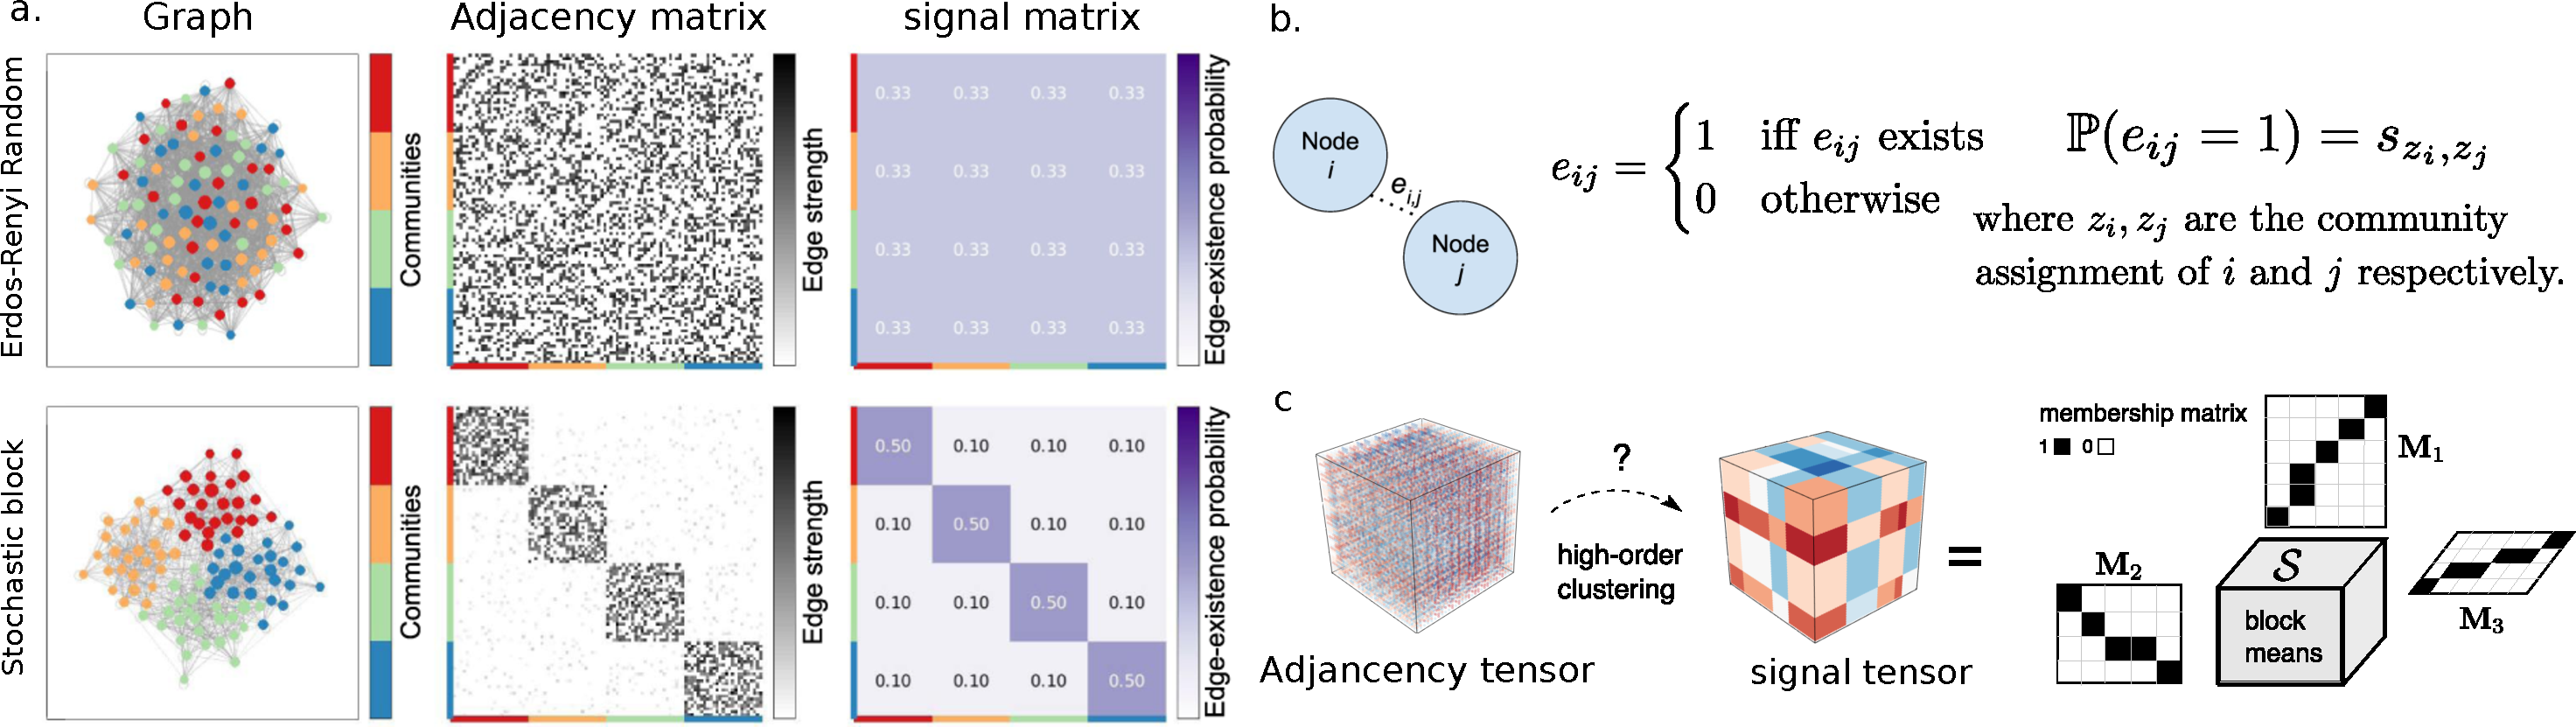
\includegraphics[width=.9\textwidth]{network1.pdf}
\caption{(a) Representation of network data using adjacency matrices (Pictures adopted from Faskowitz et al, 2018). (b) Stochastic block model for single-layer network (i.e., matrix). (c) We propose tensor extension of block model for high-order clustering in the context of multi-layer networks.}\label{fig:1}
\end{center}
\vspace{-.6cm}
\end{figure}

We propose to develop mathematical theory and scalable algorithms for tensor stochastic block models. The learning goal is to estimate multi-way connection strength tensor and community assignments from a noisy observation (see Figure~\ref{fig:1}c). We will develop a scalable higher-order Lloyd algorithm, which uses alternating optimization for parameter estimations. Our preliminary analysis shows that the tensor algorithm achieves exact recovery of communities under less stringent assumptions than existing algorithms. We aim to characterize statistical-computational trade-off for higher-order clustering, and develop proverably accurate and efficient algorithms. 

\mybox[gray!20]{
{\bf Impact and significance:} 
\begin{itemize}[leftmargin=*]
\item Establish machine learning foundations for unsupervised tensor clustering and dimension reduction. 
\item Design robust and efficient algorithms for large-scale tensor data computation. 
\item Create data-driven solutions and pipelines for tensor data analysis.
\end{itemize}
 }
 
{\bf Expected products and deliverables.} As a young PI, I have been actively contributed to several multi-institutional consortiums, in collaboration with researchers in both academics and industry. This grant will support me to further create a diverse working group. Open-source software will be released, as the fruit of the research, that benefits academia, industry, and society.

\end{document}